%%%%%%%%%%%%%%%%%%%%%%%%%%%%%%%%%%%%%
% LaTeX poster template
% Created by Nathaniel Johnston
% August 2009
% http://www.nathanieljohnston.com/2009/08/latex-poster-template/
%%%%%%%%%%%%%%%%%%%%%%%%%%%%%%%%%%%%%%

\documentclass[final]{beamer}
\usepackage[scale=0.8]{beamerposter}
\usepackage{graphicx}
\usepackage{multicol}
\usepackage{ragged2e}
\usepackage{epstopdf}
\usepackage{array}
\usepackage{tikz}
\usetikzlibrary{arrows.meta,calc,positioning,shadows}

% Typography: match the serif-heading feel of the v2 Pathways deck.
% Palatino-like body via mathpazo; keep sans for UI micro-labels.
\usepackage{mathpazo}
\usepackage[T1]{fontenc}
\usepackage{microtype}

%-----------------------------------------------------------
% Poster dimensions and columns
%-----------------------------------------------------------
\newlength{\sepwid}
\newlength{\onecolwid}
\newlength{\twocolwid}
\newlength{\threecolwid}
\setlength{\paperwidth}{36in}
\setlength{\paperheight}{24in}
\setlength{\textwidth}{0.98\paperwidth}
\setlength{\textheight}{0.98\paperheight}
\setlength{\sepwid}{0.005\paperwidth}
\setlength{\onecolwid}{0.29\paperwidth}
\setlength{\twocolwid}{0.610\paperwidth}
\setlength{\threecolwid}{0.815\paperwidth}
\setlength{\topmargin}{-1.2in}

% Theme support: the template expects a garnet color.
\definecolor{garnet}{HTML}{741947}
\usetheme{confposter}

%-----------------------------------------------------------
% Color system from the v2 Pathways presentation
%-----------------------------------------------------------
\definecolor{PathwaysCream}{HTML}{F4F2EA}
\definecolor{PathwaysBurgundy}{HTML}{741947}
\definecolor{PathwaysGreen}{HTML}{2F6F3E}
\definecolor{PathwaysSoftGreen}{HTML}{DCEAD2}
\definecolor{PathwaysSoftPink}{HTML}{EFE4EC}
\definecolor{PathwaysGray}{HTML}{5E5E5E}
\definecolor{PathwaysLightGray}{HTML}{E8E6E1}
\definecolor{PathwaysPurple}{HTML}{7B2DA0}

\setbeamercolor{background canvas}{bg=PathwaysCream}
\setbeamercolor{block title}{fg=PathwaysBurgundy,bg=PathwaysCream}
\setbeamercolor{block body}{fg=black,bg=PathwaysCream}
\setbeamercolor{block alerted title}{fg=white,bg=PathwaysBurgundy}
\setbeamercolor{block alerted body}{fg=black,bg=PathwaysSoftPink}
\setbeamercolor{item}{fg=PathwaysGreen}
\setbeamercolor{item projected}{fg=white,bg=PathwaysGreen}
\setbeamercolor{cboxb}{fg=white,bg=PathwaysBurgundy}
\setbeamerfont{block title}{series=\bfseries,size=\Large}
\setbeamerfont{block alerted title}{series=\bfseries,size=\Large}
\setbeamerfont{itemize/enumerate body}{size=\normalsize}
\setbeamerfont{itemize item}{size=\normalsize}

% Big-number metric card: heavy numeric display in burgundy, small caps label.
% Width tuned so three cards + \hfill fit a single column without overflow.
\newcommand{\metricbox}[2]{%
  \begin{tikzpicture}[baseline=(n.base)]
    \node[
      rounded corners=6pt,
      draw=PathwaysBurgundy!55!black,
      line width=1.1pt,
      fill=PathwaysSoftPink,
      text width=0.235\linewidth,
      align=center,
      inner xsep=0.3em,
      inner ysep=0.7em
    ] (n) {%
      {\color{PathwaysBurgundy}\fontsize{38pt}{40pt}\selectfont\bfseries #1}\\[0.15em]%
      {\color{PathwaysGray}\footnotesize\scshape #2}%
    };
  \end{tikzpicture}%
}

\newcommand{\phasebox}[3]{%
  \begin{tikzpicture}[baseline=(n.base)]
    \node[
      rounded corners=5pt,
      draw=#1!70!black,
      line width=1pt,
      fill=#1!12,
      text width=0.255\linewidth,
      align=center,
      inner xsep=0.4em,
      inner ysep=0.85em
    ] (n) {%
      {\color{#1!55!black}\bfseries\large #2}\\[0.2em]%
      {\small #3}%
    };
  \end{tikzpicture}%
}

\newcommand{\figcaption}[1]{%
  \vspace{-0.35em}
  {\footnotesize\itshape\color{PathwaysGray}#1}
}

\newcommand{\ragflowdiagram}{%
\resizebox{1.0\linewidth}{!}{%
\begin{tikzpicture}[
  font=\normalsize,
  node distance=0.7cm and 0.6cm,
  box/.style={draw=PathwaysGreen!60!black, rounded corners=4pt, line width=1pt,
    fill=PathwaysSoftGreen, align=center, minimum height=1.5cm, text width=3.1cm},
  db/.style={draw=PathwaysBurgundy, rounded corners=4pt, line width=1pt,
    fill=PathwaysSoftPink, align=center, minimum height=1.5cm, text width=3.1cm},
  llm/.style={draw=PathwaysPurple, rounded corners=4pt, line width=1pt,
    fill=PathwaysPurple!12, align=center, minimum height=1.5cm, text width=3.1cm},
  arr/.style={-{Stealth[length=2.6mm]}, line width=1.2pt, draw=PathwaysGreen!70!black}
]
\node[box] (q) {User\\query};
\node[box, right=of q] (embed) {Embed\\query};
\node[db, right=of embed] (db) {Supabase\\vector DB};
\node[box, right=of db] (chunks) {Retrieved\\pathway chunks};
\node[llm, right=of chunks] (llm) {LLM of\\choice};
\node[db, right=of llm] (answer) {Source-\\grounded\\response};
\draw[arr] (q) -- (embed);
\draw[arr] (embed) -- (db);
\draw[arr] (db) -- (chunks);
\draw[arr] (chunks) -- (llm);
\draw[arr] (llm) -- (answer);
\end{tikzpicture}}%
}

\newcommand{\digestdiagram}{%
\resizebox{1.0\linewidth}{!}{%
\begin{tikzpicture}[
  font=\normalsize,
  node distance=0.65cm and 0.55cm,
  stage/.style={draw=PathwaysGreen!60!black, rounded corners=4pt, line width=1pt,
    fill=PathwaysSoftGreen, align=center, minimum height=1.45cm, text width=2.95cm},
  tech/.style={draw=PathwaysBurgundy, rounded corners=4pt, line width=1pt,
    fill=PathwaysSoftPink, align=center, minimum height=1.45cm, text width=2.95cm},
  arr/.style={-{Stealth[length=2.6mm]}, line width=1.2pt, draw=PathwaysGreen!70!black}
]
\node[stage] (pdfs) {Pathway PDFs\\and modules};
\node[stage, right=of pdfs] (clean) {Clean text\\+ metadata};
\node[tech, right=of clean] (chunks) {Docling hybrid\\chunks};
\node[tech, right=of chunks] (embed) {Vectors};
\node[stage, right=of embed] (store) {Supabase\\storage};
\node[stage, right=of store] (filter) {Pathway filter\\+ citations};
\draw[arr] (pdfs) -- (clean);
\draw[arr] (clean) -- (chunks);
\draw[arr] (chunks) -- (embed);
\draw[arr] (embed) -- (store);
\draw[arr] (store) -- (filter);
\end{tikzpicture}}%
}

%-----------------------------------------------------------
% Headline with Trinity and Connecticut Children's marks.
% Matches the v2 deck: serif title in burgundy, green accent subtitle,
% gray author line, and a hairline burgundy rule flush with content.
%-----------------------------------------------------------
\setbeamertemplate{headline}{
 \leavevmode
 \vspace*{-0.5cm}
  \begin{columns}[c,totalwidth=\textwidth]
   \begin{column}{0.16\textwidth}
     \centering
     
\includegraphics[height=3.4cm]{trinityLogo.png}
   \end{column}
   \begin{column}{0.68\textwidth}
    \centering
    {\color{PathwaysBurgundy}\fontsize{68pt}{72pt}\selectfont\textbf{\inserttitle}\\[0.15ex]}
    {\color{PathwaysGreen}\Large\itshape Intelligent document search for pediatric clinical decision support\\[0.4ex]}
    {\color{PathwaysGray}\large \insertauthor\\[0.25ex]}
    {\color{PathwaysGray}\normalsize \insertinstitute}
   \end{column}
   \begin{column}{0.16\textwidth}
     \centering
     
\includegraphics[width=0.85\linewidth]{pathways_assets/ct_childrens_logo.png}
   \end{column}
  \end{columns}
 \vspace{0.06in}
 \centering
 {\color{PathwaysBurgundy}\rule{0.97\textwidth}{0.07cm}}
 \vspace{0.04in}
}

% Cream-on-cream block titles with a burgundy underline rule. Left-aligned to
% give the poster a cleaner editorial feel (matches the deck's left-aligned
% section titles). Extra top padding prevents the previous block's body from
% crowding the next block's title.
\setbeamertemplate{block begin}
{
  \par\vskip1.4ex
  \begin{beamercolorbox}[colsep*=0ex,dp={1.4ex},leftskip=0pt]{block title}
    \usebeamerfont{block title}\Large\textbf{\insertblocktitle}
    \vskip0.15cm
    {\color{PathwaysBurgundy!80}\rule{\linewidth}{0.055cm}}
  \end{beamercolorbox}
  {\parskip0pt\par}
  \usebeamerfont{block body}
  \vskip-0.15cm
  \begin{beamercolorbox}[colsep*=0ex,vmode]{block body}
  \justifying
}

%-----------------------------------------------------------
% Title information
%-----------------------------------------------------------
\title{The Pathways Project}
\author{Kwaku Agyapong \textquoteright 26 \, \textperiodcentered \, Kitae Hwang \textquoteright 26}
\institute{CT Children's Medical Center \, $\times$ \, AIQUI Sandbox \hspace{0.8em} | \hspace{0.8em} Advisor: Kenneth Kousen \hspace{0.8em} | \hspace{0.8em} Trinity College Senior Seminar}

\begin{document}
\begin{frame}[t]
\begin{columns}[t]

% ------------------------ Column 1 ------------------------
\begin{column}{\sepwid}\end{column}
\begin{column}{\onecolwid}

\begin{alertblock}{Project Goal}
\normalsize
Build a pathway-aware RAG chatbot that helps clinicians and staff search Connecticut Children's pediatric clinical pathways with fast, relevant, and source-grounded responses.
\end{alertblock}
\vskip1ex

\begin{block}{Problem and Use Case}
\normalsize
Clinical pathways are dense, multi-document resources. The project focuses on turning guideline libraries into a searchable assistant that keeps answers tied to the selected pathway.

\vspace{0.8em}
\centering
\metricbox{67}{pathways}\hfill
\metricbox{30}{pages / pathway}\hfill
\metricbox{2010}{source pages}

\vspace{0.9em}
\justifying
\textbf{Why this matters}
\begin{itemize}
\item Clinical users need quick navigation across algorithms, educational modules, and related pathway PDFs.
\item General-purpose LLM answers are not enough; retrieval must be limited to the selected clinical context.
\item The system should reduce document-hunting while preserving clinical judgment and source visibility.
\end{itemize}
\end{block}

\begin{block}{Clinical Pathway Source}
\centering

\includegraphics[width=0.88\linewidth,height=0.175\paperheight,keepaspectratio]{pathways_assets/clinical_pathway_crop.png}
\figcaption{Anaphylaxis pathway: triage, treatment, and disposition algorithm.}
\end{block}

\begin{block}{Success Criteria}
\normalsize
\begin{itemize}
\item Search is scoped to a chosen pathway, not the open web.
\item Retrieval returns precise chunks with pathway and page metadata.
\item Answers are presented alongside their source context.
\item Monitoring and feedback enable iterative quality improvement.
\end{itemize}
\end{block}

\end{column}

% ------------------------ Column 2 ------------------------
\begin{column}{\sepwid}\end{column}
\begin{column}{\onecolwid}

\begin{block}{Baseline RAG Pattern}
\normalsize
Retrieval augmented generation turns a user query into a vector search over embedded documents, then gives the LLM the retrieved context before it answers.

\vspace{0.5em}
\centering
\ragflowdiagram
\figcaption{Query embedding $\rightarrow$ vector search $\rightarrow$ retrieved context $\rightarrow$ response generation.}

\vspace{0.7em}
\justifying
\textbf{Why not just a general-purpose LLM?}
\begin{itemize}
\item A general LLM hallucinates specifics; clinical answers must be traceable to a pathway document.
\item Open-web retrieval returns irrelevant or outdated guidance instead of the hospital's own pathway.
\item Ground-truth sources at CT Children's live in versioned PDFs, not in the pre-training corpus.
\end{itemize}
\end{block}

\begin{block}{Heavy-Digestion Pipeline}
\normalsize
Raw PDFs carry broken tables, split paragraphs, and embedded figures that a direct ingest would dump into the index as noise. The heavy-digestion pipeline does the expensive document work \emph{once}, up front, so retrieval at query-time is fast and precise.

\vspace{0.5em}
\centering
\digestdiagram
\figcaption{Document transformation $\rightarrow$ chunking $\rightarrow$ embedding $\rightarrow$ vector storage $\rightarrow$ pathway filtering.}
\end{block}

\begin{alertblock}{Design Principle}
\normalsize
Do more document work \emph{before} retrieval, so the chatbot can do less guessing \emph{during} clinical question answering.
\end{alertblock}

\begin{block}{Direct Ingest vs.\ Heavy Digest}
\small
\setlength{\tabcolsep}{0.4em}
\renewcommand{\arraystretch}{1.15}
\begin{center}
\begin{tabular}{@{}p{0.26\linewidth} p{0.30\linewidth} p{0.32\linewidth}@{}}
\textbf{\color{PathwaysGray}\scshape dimension}
 & \textbf{\color{PathwaysBurgundy}Direct ingest}
 & \textbf{\color{PathwaysGreen}Heavy digest (ours)}\\
\hline
Chunking     & fixed char windows & document-aware ($\sim$512 tok) \\
Metadata     & none / filename    & pathway, section, page \\
Retrieval    & whole corpus       & pathway-filtered \\
Fidelity     & lossy, generic     & traceable, specific \\
\end{tabular}
\end{center}
\end{block}

\end{column}

% ------------------------ Column 3 ------------------------
\begin{column}{\sepwid}\end{column}
\begin{column}{\onecolwid}

\begin{block}{Prototype Interface}
\normalsize
The demo lets a user select a pathway, ask a question, and inspect the source PDF in one workflow.

\vspace{0.5em}
\centering
\begin{minipage}[t]{0.48\linewidth}
\centering
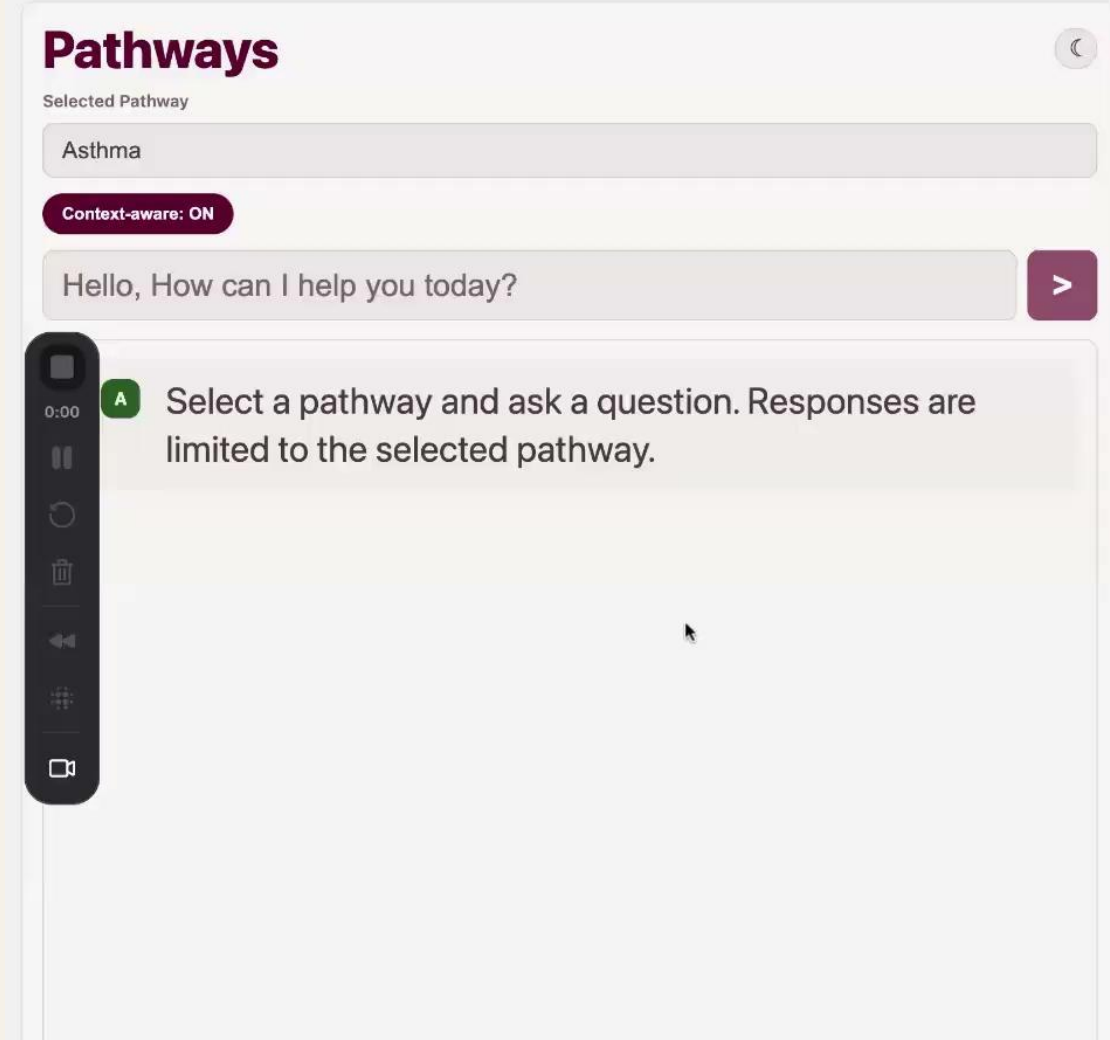
\includegraphics[width=\linewidth,height=0.145\paperheight,keepaspectratio]{pathways_assets/demo_chat_crop.png}\\[0.15em]
{\scriptsize\color{PathwaysGray}Pathway-scoped chat, context-aware mode}
\end{minipage}\hfill
\begin{minipage}[t]{0.48\linewidth}
\centering
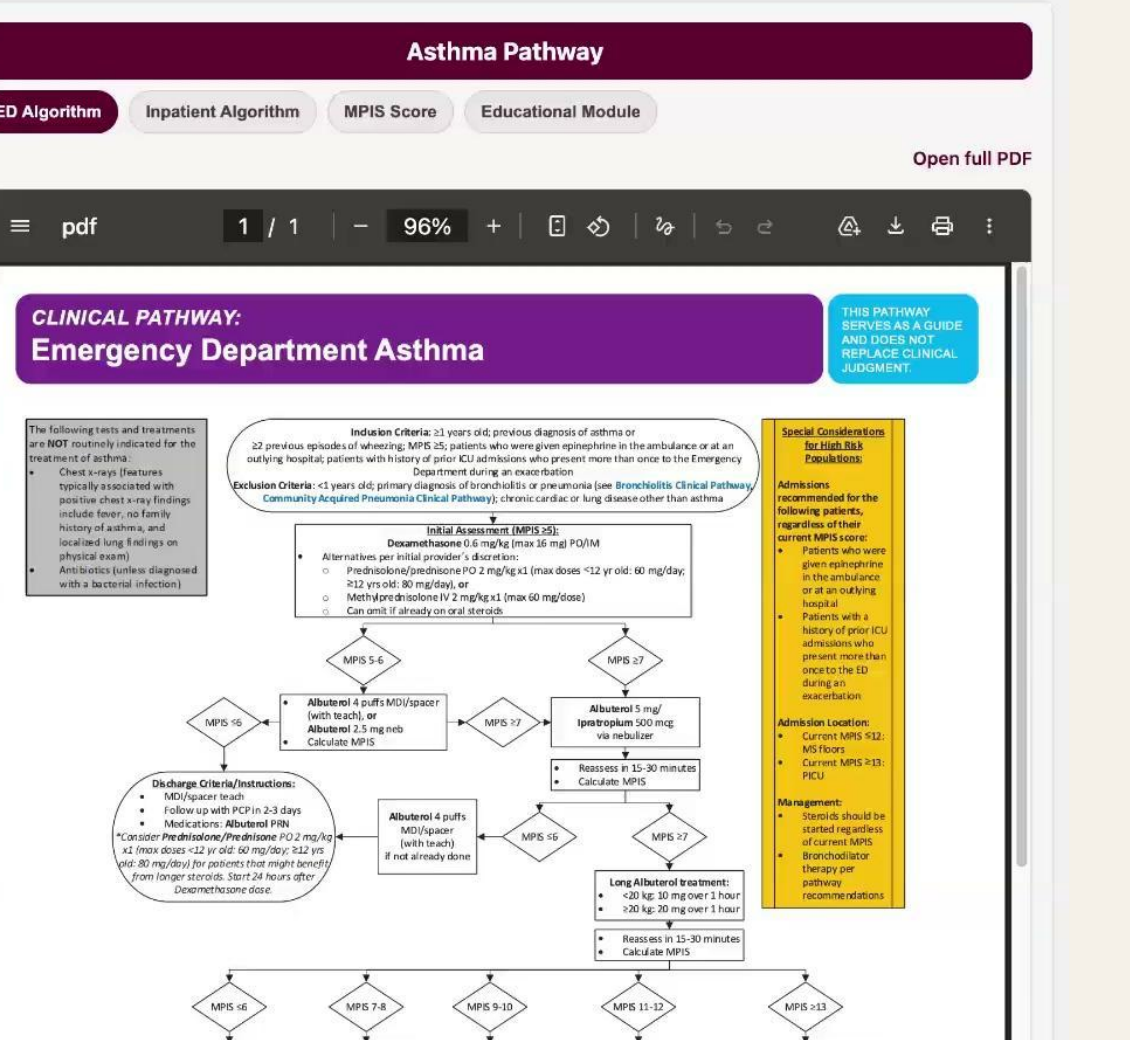
\includegraphics[width=\linewidth,height=0.145\paperheight,keepaspectratio]{pathways_assets/demo_pdf_crop.png}\\[0.15em]
{\scriptsize\color{PathwaysGray}Embedded PDF viewer, tabbed modules}
\end{minipage}

\vspace{0.7em}
\justifying
\begin{itemize}
\item Pathway selection constrains retrieval to relevant source material.
\item Context-aware mode supports natural follow-up questions.
\item PDF tabs expose ED/inpatient algorithms, scores, and educational modules.
\end{itemize}
\end{block}

\begin{block}{Answer Quality Across Rounds}
\small
Three evaluation rounds against a fixed 15-question clinical benchmark (Migraine, CAP, Asthma~ED). Each round changed one layer of the stack---chunking, embedding, then pathway tagging---so gains could be attributed to specific decisions.

\vspace{0.5em}
\setlength{\tabcolsep}{0.3em}
\renewcommand{\arraystretch}{1.25}
\begin{center}
\begin{tabular}{@{}p{0.42\linewidth} C{0.15\linewidth} C{0.15\linewidth} C{0.17\linewidth}@{}}
\textbf{\color{PathwaysGray}\scshape question}
 & \textbf{\color{PathwaysGray}\scshape R1}
 & \textbf{\color{PathwaysGray}\scshape R2}
 & \textbf{\color{PathwaysGray}\scshape R3}\\
\hline
CAP: antibiotic course length        & 5\%  & 90\% & \textbf{92\%} \\
CAP: admission criteria              & 10\% & 35\% & \textbf{85\%} \\
Asthma: MPIS score calculation       & 58\% & 65\% & \textbf{80\%} \\
\end{tabular}

\vspace{0.3em}
{\footnotesize\color{PathwaysGray}\itshape R1: MiniLM 384-dim, fixed chunks. R2: MedCPT 768-dim, semantic chunks + Claude image-to-text. R3: MedEmbed 1024-dim + pathway tagging.}
\end{center}

\vspace{0.4em}
\justifying
\begin{itemize}
\item \textbf{R1$\rightarrow$R2: the step change.} Semantic chunking and a clinical encoder drove the biggest gains---content trapped in figures was recovered by Claude image-to-text.
\item \textbf{R2$\rightarrow$R3: structure over dimensionality.} 1024-dim was marginal; \textbf{pathway tagging} unlocked CAP admission criteria by routing queries to the right document subset.
\item \textbf{Remaining failures are semantic}, not structural---ambiguous clinical terms need query-side prompting.
\end{itemize}
\end{block}

\begin{block}{Takeaways}
\normalsize
\justifying
\begin{itemize}
\item \textbf{Clinical alignment} --- communication with CT~Children's.
\item \textbf{Prior art} --- learning from Seattle and Arizona.
\item \textbf{Impact} --- building something that matters.
\end{itemize}

\vspace{0.3em}
\textbf{Next step:} validate retrieval quality against pathway-specific questions, then connect monitoring and feedback data back into the document-processing pipeline.
\end{block}

\end{column}
\begin{column}{\sepwid}\end{column}

\end{columns}
\end{frame}
\end{document}
